\documentclass[11pt]{article}
\usepackage[utf8]{inputenc}
\usepackage{geometry}
\usepackage{graphicx}
\usepackage{hyperref}
\usepackage{amsmath}
\usepackage{listings}
\usepackage{xcolor}
\usepackage{float}

% Set page margins
\geometry{a4paper, margin=1in}

% Set up code listing style
\lstset{
    basicstyle=\ttfamily,
    commentstyle=\color{gray},
    keywordstyle=\color{blue},
    stringstyle=\color{red},
    showstringspaces=false,
    captionpos=b
}

\title{Development of a Sudoku Solver: C1 Research Computing Coursework}
\author{Vishal Jain}
\date{\today}

\begin{document}

\maketitle

\tableofcontents

\newpage

\section{Introduction}

\begin{quote}
    "Sudoku is a denial of service attack on human
  intellect" - Ben Laurie
\end{quote}

This report details the development of a Sudoku solver inline with the requirements of the C1 Research Computing coursework. The programme takes as input an incomplete grid in the form of a text file with a 9x9 grid of numbers with zero representing unknown values and `|`,`+`,`-` separating cells and , i.e.:


\begin{verbatim}
    $ cat input.txt
    000|007|000
    000|009|504
    000|050|169
    ---+---+---
    080|000|305
    075|000|290
    406|000|080
    ---+---+---
    762|080|000
    103|900|000
    000|600|000
    \end{verbatim}

and outputs the completed grid in the same form.

\subsection{Background and motivation}

Sudoku, a logic-based combinatorial number-placement puzzle, presents a paradigmatic example of a constraint satisfaction problem (CSP), a class of problems fundamental to the field of computer science. The puzzle's structure, consisting of a 9x9 grid divided into subgrids, adheres to stringent placement rules, thereby embodying the essence of CSPs where the objective is to find a solution that satisfies all given constraints.

This project, centered on the development of a Sudoku solver, is primarily motivated by the pedagogical value inherent in addressing such a well-defined and constrained problem space. Sudoku solvers exemplify the application of algorithmic strategies to a finite, yet non-trivial problem domain. This aligns with the core objectives of the C1 Research Computing coursework, which emphasizes the development of computational solutions that are both efficient and effective.

The logical structure and deterministic nature of Sudoku make it an ideal candidate for exploring various algorithmic approaches, from brute-force methods to more sophisticated heuristic algorithms. Furthermore, the project offers a platform for implementing and refining software development practices, particularly in areas such as code clarity, modular design, and performance optimisation.

In essence, the construction of a Sudoku solver serves not only as an exercise in algorithm implementation but also as a microcosm for broader software development and computational problem-solving skills. It provides a controlled environment to experiment with and evaluate different computational strategies, thereby contributing to a deeper understanding of both the specific problem of Sudoku and the general principles of algorithm design and optimization in computer science.
\section{Problem Decomposition}
To architect the Sudoku solver program, an initial flowchart was constructed to map out the high-level logical sequence. Each step of the flowchart was assigned a color based on its independence; steps that could be altered without impacting preceding steps received a unique color, whereas related, interdependent steps shared the same color. This method helped identify distinct, modular components within the program's workflow. The resulting color-coded flowchart is presented in Figure \ref{fig:solver_flowchart}.
\begin{figure}[H]
\centering
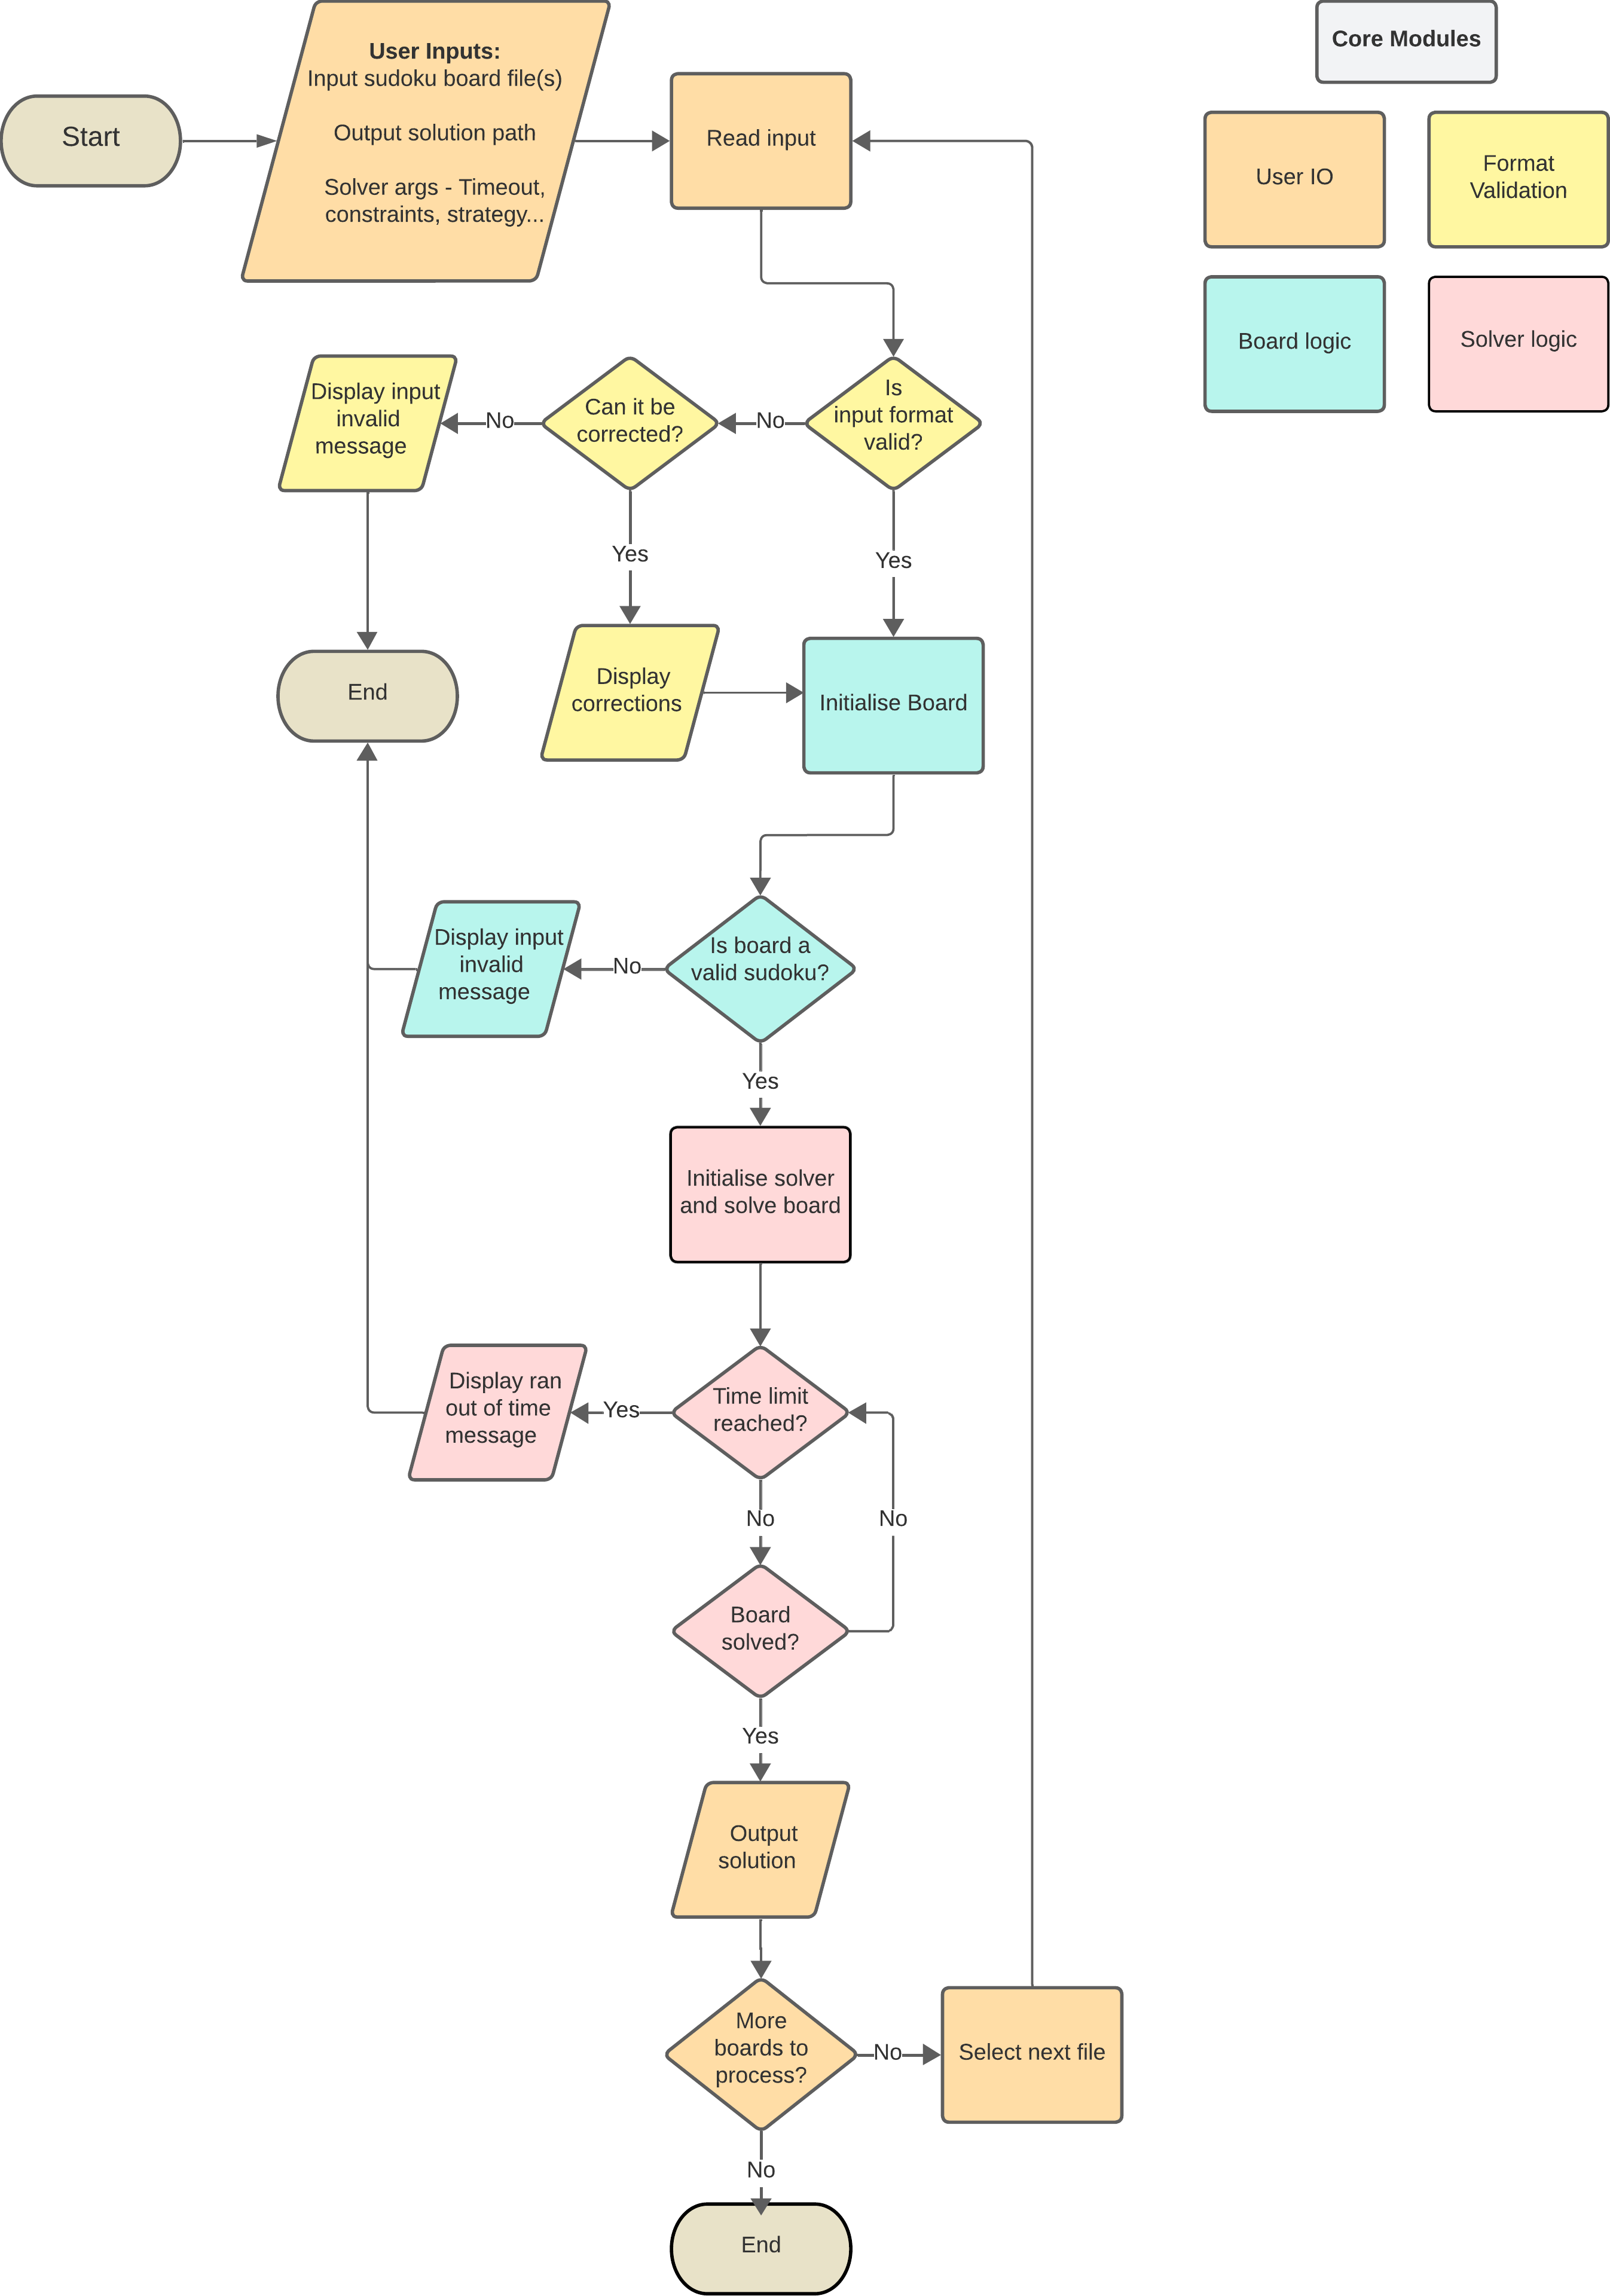
\includegraphics[width=0.82\textwidth]{figs/solver_flowchart.png}
\caption{High-level flowchart of the Sudoku solver program, illustrating the initial conceptual design. Functionally related modules are color-coded: orange for user interaction, yellow for format validation, cyan for board logic, and pink for solver logic components.}
\label{fig:solver_flowchart}
\end{figure}

The analysis led to the identification of the following key modular components in the Sudoku solver:

\begin{itemize}
\item \textbf{User IO:} Responsible for user interaction and input/output processing.
\item \textbf{Format Validation:} Ensures the correctness of the input format.
\item \textbf{Board Logic:} Manages the internal representation and manipulation of the Sudoku board.
\item \textbf{Solver Logic:} Implements the algorithms to solve the Sudoku puzzle.
\end{itemize}

Moreover, the following areas were identified as key areas in which the program might be extended in the future:
\begin{itemize}
\item Introduction of additional input formats.
\item Integration of more sophisticated solver algorithms.
\item Adaptation to alternative Sudoku board representations.
\end{itemize}

Each module is purposefully designed to operate independently, minimising inter-module dependencies. This approach not only facilitates ease of modification and maintenance but also allows for isolated testing and enhancement of individual components. Error handling is strategically implemented within each module, focusing on specific functional requirements. To ensure system-wide robustness, some error checks are intentionally overlapped across modules. The following sections will delve into the scope, design, implementation, and constraints of each module, along with a discussion on their potential for future enhancements.
\section{User IO}
\subsection{Scope}
The User IO module is responsible for the interaction between the user and the program. It is the only module that interacts with the user, and it is responsible for the following tasks:
\begin{itemize}
    \item Collecting user input.
    \item Validating user input.
    \item Showing the output of the program.
    \item Saving the output of the program.
\end{itemize}

\subsection{Design and Prototyping}
It is ironic that this module which is presented first was actually the last module to be implemented since it required some time spent playing around with the other modules and trying to figure out the best way to call them.

The first step when designing this module was to think about what the were the ways in which the user might want to call the sudoku solver. 

It should be easy to take an input sudoku board file and solve it, you do not want to specify many parameters each time just to run a quick solving task. 

While designing the program, often a board would be found online and having to save it to a file first and pointing the solver to it was a repeated pain. It is therefore desirable to be able to take in a string of a sudoku board from main.primarily

the module should also be independant of changes to the back end. If a new solver is added or if support for a new input format is added on the back end, the user should be able to simply select these as options from the cli args.

There are 2 ways in which the script could be called. One is for single input, where a single sudoku board is passed as input and a solution is desired.

Another is for batch testing where one may want to test the performance of a new solver or board representation against a dataset of boards.

In the case of batch testing there are also some other desires, eg the desire to save outputs, output time statistics. 

Currently at the time of writing this report the solvers are quite basic and only require a single argument to be initialised - the timeout arg. However, in the future the solvers may grow more complex and as such the number of parameters required to initialise them may grow and may become more specific to a solver. As such in the future the best way to handle this would be to put all solver specific parameters in a config file and load that config file. There is a specific space in the main.py where this logic lives. 

Another desired feature is reproducability of runs, especially when trying to compare performances of different versions of the solver, it should be possible to reproduce a run from the output summary json. As such the git commit hash and arguments of the run are saved as well.

The main function works as following. It was decided not to implement the module as a class but rather as a main.py script which has functions instead of methods. <justify this>

The $main.py$ script collects user args via arg parse. It is made so that rapid prototyping is possible where if a user just wants to quickly solve a puzzle the only required arguments are the puzzle input. if the puzzle input is set as a string then the optional $--input_type$ flag. must be set to str. 

This is the fastest way to check that a given solver 

% Uncomment the following two lines if you have references
%\bibliographystyle{plain}
%\bibliography{references}

\end{document}
